\documentclass[11pt]{article}

\usepackage{graphicx}
\usepackage[sorting=none]{biblatex}
\usepackage[margin=1in]{geometry}
\usepackage[colorlinks=true]{hyperref}
\usepackage{amsmath}
\usepackage{amssymb}
\usepackage[format=plain, labelfont=it, font=footnotesize, labelsep=period]{caption}
\usepackage{caption}
\usepackage{subcaption}
\usepackage{multicol}
\usepackage{wrapfig}
\usepackage{float}
\usepackage{lipsum}

\addbibresource{references.bib}

\title{Pendulum Lab Report II}
\author{Kevin (Zerui) Wang}
\date{\today}


\begin{document}

\pagenumbering{gobble}
\maketitle
\tableofcontents
\newpage

\pagenumbering{arabic}




\begin{multicols}{2}
\section{Introduction}
{\color{blue}The purpose of this lab report is to evaluate the accuracy of various theoretical models used to predict the behaviour of a simple pendulum, namely the relationship between period and release angle, amplitude and time, period and length, and Q factor and length.}

\section{Background} \label{Background}
A simple pendulum can be defined as a weight suspended via a flexible string, below a pivot point to which it swings back and forth freely along a plane that contains the pivot point. The length of the pendulum is defined as the distance from the pivot point to the weight's center of mass. For a simple pendulum of length $L$ experiencing a downwards force due to gravity $g$, the period $T$, for a release angle $\theta$, is given by the following equation \cite{the-simple-pendulum}, provided that the mass of the string is negligible compared to the mass of the weight:
\begin{equation} \label{eq:l-over-g}
    T = 2\pi \sqrt{\frac{L}{g}}
\end{equation}



More realistically, the behavior of an ideal pendulum assuming no energy loss due to friction can be modelled with a second order differential equation of $\theta$ with respect to $t$:
\begin{equation} \label{eq:diffeq-pendulum}
    \frac{d^2\theta}{dt^2} + \frac{g}{L}\sin{\theta} = 0
\end{equation}
where the solution $\theta(t)$ cannot be easily represented in terms of elementary functions \cite{no-elementary-fns}. Accordingly, the derived formula for $T(\theta)$ from Equation \ref{eq:diffeq-pendulum} is best described as an infinite series \cite{no-elementary-fns-2}:
\begin{align} \label{eq:power-series-derived}
\begin{split}
    T(\theta) &= 2\pi\sqrt{\frac{L}{g}} \left(1 + \frac{1}{4}\sin^2\frac{\theta}{2} \right. + \\
    &\phantom{{}=}\left. \frac{9}{64}\sin^4\frac{\theta}{2} + \frac{225}{2304}\sin^6\frac{\theta}{2} + \ldots \right)
\end{split}
\end{align}


Equation \ref{eq:power-series-derived} essentially equals Equation \ref{eq:l-over-g} when $\theta$ is extremely small. This is known as the small angle approximation of a pendulum and it holds (implying simple harmonic motion also holds) for $|\theta| \lesssim 20^{\circ}$ \cite{the-simple-pendulum}. When $\theta$ is in this range, $\sin\theta \approx \theta$. Additionally, all previous models demonstrate that pendulum period does not depends on mass of the weight.

Another way to realistically model a pendulum is to incorporate dampening from frictional forces given by the following equation \cite{damped-oscillations}
\begin{equation} \label{eq:damped-harmonic-oscillator}
    \theta(t) = \theta_0 e^{-{t/\tau}} \cos\left(2\pi\frac{t}{T} + \phi_0\right)
\end{equation}
where:
{
\setlength{\abovedisplayskip}{2.5pt}
\begin{flalign*}
    \quad \theta_0 &= \text{initial release angle in radians} & \\ % \\[-3pt] for paragraphs
    % \quad &\phantom{{}={}} \text{ayo continuation br}\\
    \quad T &= \text{pendulum's period} & \\
    \quad \phi_0 &= \text{angular phase shift} & \\
    \quad \tau &= \text{decay constant governing damping} &
\end{flalign*}
}

It can be inferred from Equation \ref{eq:damped-harmonic-oscillator} that $T$ is constant for this model, implying the presence of small angle approximation. Additionally, removing the cosine term yields the amplitude-time graph:
\begin{equation} \label{eq:amplitude-function}
    A(t) = \theta_0 e^{-{t/\tau}}
\end{equation}

In order to quantify a pendulum's damping, its Q factor may be used. The Q factor measures how damped an oscillator is and is defined as follows. \cite{pnp-physics}:
\begin{equation} \label{eq:q-factor-formula}
    Q = \pi\frac{\tau}{T}
\end{equation}

The Q factor is also defined by the amount of oscillations it takes for the pendulum's amplitude to decay to $e^{-\pi} \approx 4\%$ of its original amplitude during release. Qualitatively, when the Q factor is large, the pendulum comes to rest slower. When the Q factor is small, the pendulum comes to rest quicker.

\newpage

\section{\mbox{Period and Release} \\ Angle}

\subsection{Experimental Setup}
The initial setup for the pendulum was made by first attaching a protractor on a desk. The pendulum, made by tying a piece of cotton string around a stainless steel quick link {\color{blue} that was aligned to match the $90^{\circ}$ mark on the pendulum. Extra tape was also used to reinforce the pivot point, which was made to be collinear to the $0^{\circ}$ and $180^{\circ}$ markings.} An image of the experimental setup is shown below:

\begin{figure}[H]
    \centering
    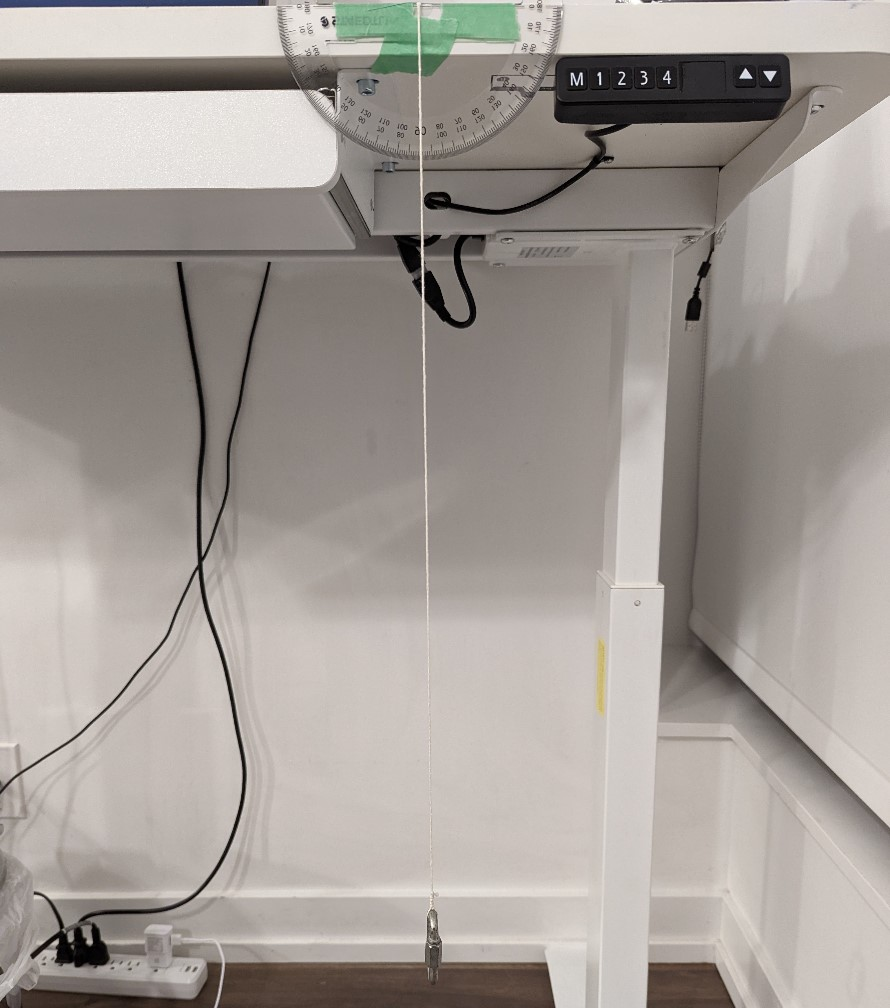
\includegraphics[width=\linewidth]{../figures/exp_setup1.jpg}
    \caption{\centering Picture of experimental setup for period vs. release angle data collection}
    \label{fig:figure 1}
\end{figure}

\subsection{Data} \label{subsec 3.2 Data}
The data collected for the period vs. release angle graph is shown in the plot below:

\begin{figure}[H]
    \centering
    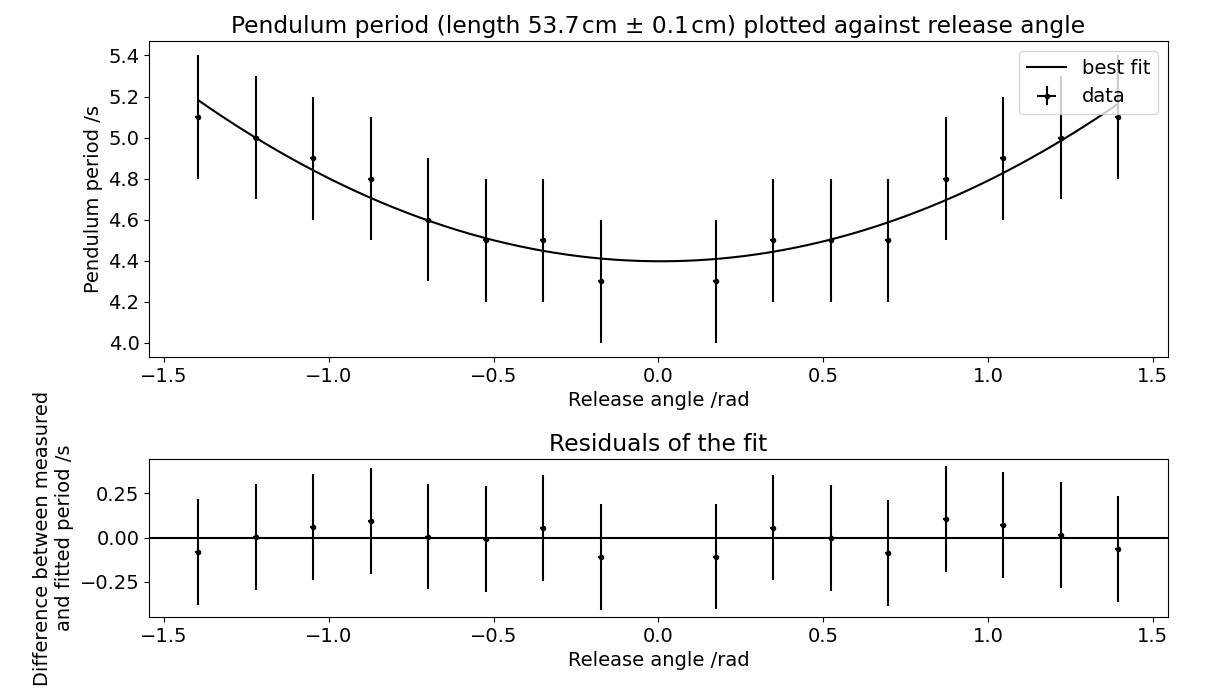
\includegraphics[width=\linewidth]{../figures/period_vs_release_angle.png}
    \caption{\centering Period plotted against release angle of the setup in Figure \ref{fig:figure 1}}
    \label{fig:figure 2}
\end{figure}

All data collected for this graph were done without the need for tracking software. {\color{blue}In total, 8 angles were recoded from both sides of the pendulum, starting from $10^\circ$ and taking increments of $10^\circ$ up to $80^\circ$}. The uncertainty for the protractor (measured by eye) was taken to be the smallest increment, $0.5^{\circ}$ converted to radians, and the period uncertainty was taken to be the average human reaction time, $0.25\,\text{s}$ \cite{reaction-time} {\color{blue} since it is greater than the uncertainty of a stopwatch. The period itself was measured by recording the pendulum for 3 swings and dividing the total time by 3. The maximum height was taken as the reference point because there would be less certainty in the pendulum's position (lower speed).}

\subsection{Analysis}
According to Section \ref{Background}, {\color{blue} if $|\theta| \lesssim 20^{\circ}$, then a line of best fit with slope 0 would be expected, which is observed to happen for the 4 closes points plotted from a release angle of $0^\circ$. However, as the release angle increases, the overall trend deviates from Equation \ref{eq:l-over-g} and takes on more of a parabolic shape which can be modelled by a quadratic power series, which corresponds to the best fit line from Figure \ref{fig:figure 1}:}
\begin{equation} \label{eq:power series}
    T_0(1 + B\theta_0 + C\theta_0^2)
\end{equation}
where $T_0$ represents the period, $\theta_0$ the release angle and $B$ and $C$ some arbitrary constants. {\color{blue}Since the $r^2$ value is relatively close to 1, the residuals are both small and consistent, and the graph passes through all error bars, this fit would be a valid representation of the trend. Additionally, the uncertainty for $T_0 = 0.03$, $B = 0.005$ and $C = 0.007$, calculated through fitting the trendline with a Python program.

The terms $B$ and $C$ are also significant because they describe the symmetry of parabola and how much it deviates from the trend described in Equation \ref{eq:l-over-g}. If $B$ does not equal 0, the parabola will not be centered at $\theta = 0$. Since the experimentally determined value of B is smaller than its uncertainty, it suffices to say that $B = 0$, which implies symmetry in the graph. On the other hand, if $C = 0$, then the line of best fit will have slope 0. However, this was determined experimentally to not be the case.


Lastly, the residuals shown on the graph do not suggest much asymmetry regarding the pendulum as the negative release angles appear symmetrical when compared to positive release angles. However, a single-stringed pendulum tends to spin in an elliptical fashion when released, affecting accurate measurements.

Thus, it can be concluded that the pendulum period depends on release angle.}

\end{multicols}
\newpage

\section{Finding the Q Factor} \label{Finding the Q Factor}

\subsection{Experimental Setup}
{\color{blue}
A single-stringed pendulum tends to spin in an elliptical fashion when released. Not only does this violate the way a pendulum was defined in Section \ref{Background}, elliptical orbits may also lead to inaccurate measurements. To correct for this,} a degree of freedom was removed from the pendulum by threading a string through the stainless steel quick link and fastening the 2 strings in 2 locations to form the shape of a ``V''. The pendulum would then swing back and forth in the plane perpendicular to the ``V'' {\color{blue} where the pivot lies directly above the string. Lego pieces were used to prevent the risk of the string slipping under the tape and a protractor was taped directly above the weight. Extra caution was taken to ensure that the center of the protractor aligned with the 2 intersection points between the string and the legos, which lined up with the camera lens. Shown below is a side and front view of the new setup:}
\begin{figure}[!hptb]
    \centering
    \begin{subfigure}{0.49\textwidth}
        \centering
        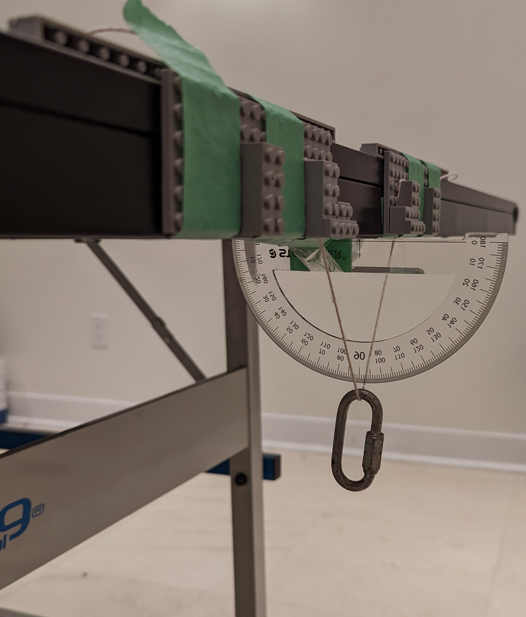
\includegraphics[width=\textwidth]{../figures/exp_setup3_angle.png}
    \end{subfigure}
    \hfill
    \begin{subfigure}{0.49\textwidth}
        \centering
        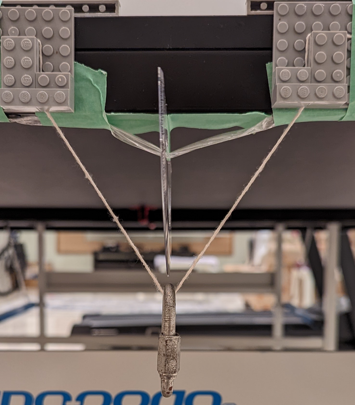
\includegraphics[width=\textwidth]{../figures/exp_setup3_front.png}
    \end{subfigure}
    \caption{\centering Improved version of the pendulum used to determine Q factor. Note: this is actually version 3 of the pendulum. Issues that arose with version 2 will be discussed later in this section. Version 2 was also double-stringed}
    \label{fig:figure 3}
\end{figure}
\newpage

\subsection{Data}
{\color{blue}
The Q factor can be determined by plotting the amplitude-time graph, as shown below:
}

\begin{figure}[!hptb]
    \centering
    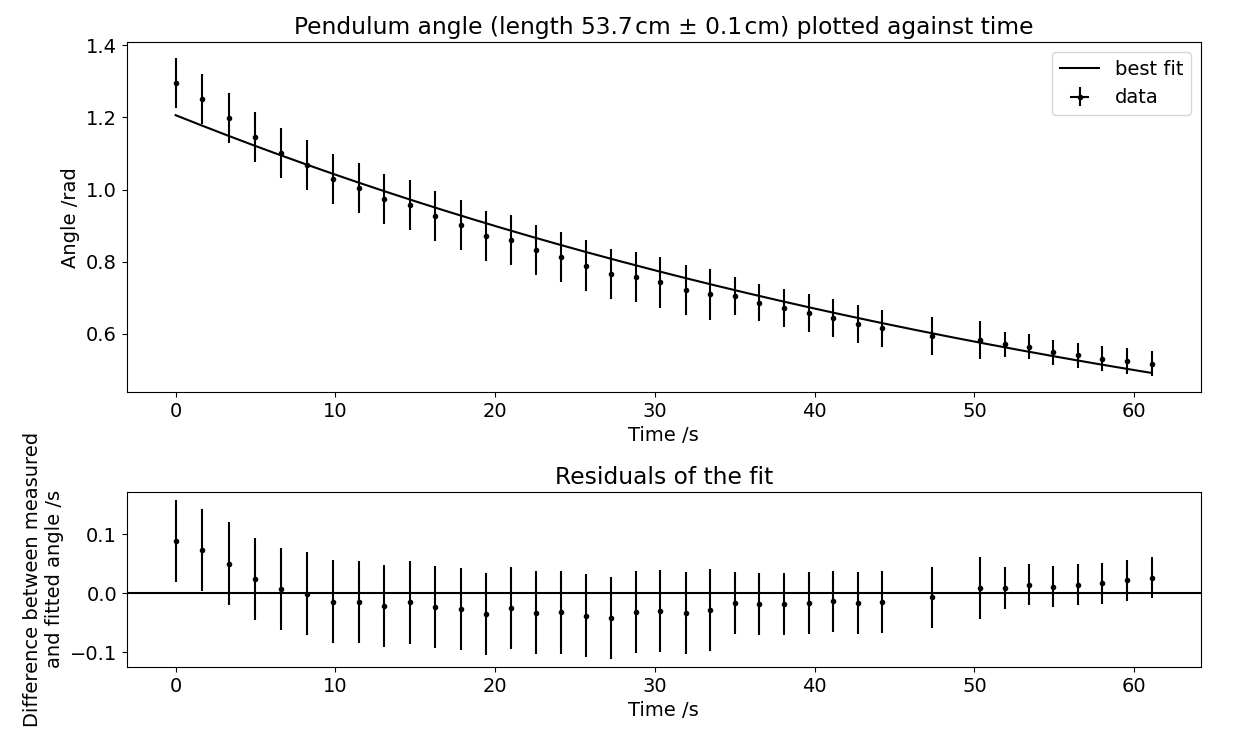
\includegraphics[width=\textwidth]{../figures/max_amplitude_vs_time.png}
    \caption{\centering Graph of maximum amplitude vs. time}
    \label{fig:figure 4}
\end{figure}

{\color{blue}
The pendulum was released from an angle of approximately $20^\circ$ to ensure the period stays constant as it is oscillating. The first version of this graph was generated with an initial release angle of 60 degrees, which resulted the period to decrease with time, producing an inaccurate Q factor. This pendulum (version 2) has since been deconstructed.

To calculate the amplitudes, the length of the video was first divided into 15\,-\,20 equal intervals. For every interval, a few frames were advanced or reversed until the closest maximum amplitude could be determined.

\newpage

The uncertainty for each angle was measured in Tracker \cite{tracker} at the frame where $\theta$ reached a maximum. Due the double-stringed setup, two strings will appear in the frame. The angle was taken to be the midpoint of the region that the strings formed and the uncertainty half of the total angle of the region. An image of angle calculation is shown below:

\begin{figure}[!hptb]
    \centering
    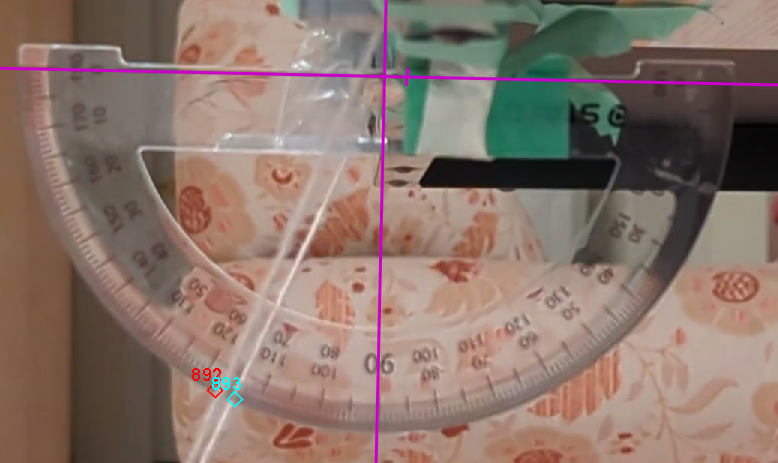
\includegraphics[width=\textwidth]{../figures/tracker.png}
    \caption{\centering Angle determination in Tracker. The red and blue diamonds represents the upper and lower bound of the angle, represented in xy coordinates relative to the pink axes, which can be converted to angles.}
    \label{fig:figure5}
\end{figure}

By using Tracker, }the uncertainty for period can be decreased from 0.25\,s to 0.03\,s, which equals to the frame rate. This is because Tracker allows the frame-by-frame playback and pausing of a video, especially at a maximum amplitude. {\color{blue}Period itself is measured by converting the number of frames taken for 5 swings into seconds, and dividing that number by 5.}

Lastly, the uncertainty for time was taken to be {\color{blue}1/30} where {\color{blue}30} represents the frame rate (fps) of the video.


\subsection{Analysis}
{\color{blue}
The best fit equation in Figure \ref{fig:figure 4} is modelled by Equation \ref{eq:amplitude-function}. The uncertainty for $\theta_0 = 0.004$ and $\tau = 2$. Simply observing the graph reveals a plausible for the the data. This is reinforced by the high $r^2$ value and small and consistent residuals.

Given Equation \ref{eq:q-factor-formula}, $T = 1.11 \pm 0.03$ for this pendulum length and $\tau = 170$, the Q factor is calculated to be $480 \pm 5$, taking on the higher percent uncertainty of $T$ and $\tau$.
Another way of determining the Q factor is by counting the number of oscillations as outlined in Section \ref{Background}. However, this method of determining the Q factor is suboptimal due to the nature of the exponential decay function.

[i dont think i ever need this section anymore] When the amplitude $A(t)$ decays to $e^{-\pi}\,\%$ of its original amplitude, the rate at which $A(t)$ changes decreases significantly. Given the value of amplitude $A_Q$ that corresponds to the time $t_Q$ when $A(t_Q) = e^{-\pi}\theta_0$, a large range of Q factors will satisfy a region of $A(t)$ around $t_Q$ bounded by the uncertainty values of $A_Q$. Additionally, the exact value of $e^{-\pi}\theta_0$ may  not correspond to any of the amplitudes but rather some angle in between two peaks. For example, if $A_Q + 0.009 = A(t)$ (Angle uncertainty from Subsection \ref{subsec 3.2 Data}), $t = 465\,\text{s}$, and if $A_Q - 0.009 = A(t)$, $t = 651\,\text{s}$. Thus, an upper and lower bound for $t_Q = 534\,\text{s}$, has been defined. Thus, Q and its uncertainty can then be found by dividing by the period and taking the larger percent uncertianties of both bounds, resulting in $Q = 480 \pm 90$ using the counting method.
SHEEESH the q factor and the counting method are pretty accurate (in terms of raw value) -> this implies that tracking pendulum this was is not flawed.
}

%%%%%%%%%%%%%%%%%%%%%%%%%%%
%%%%%%%%%%%%%%%%%%%%%%%%%%%
%%%%%%%%%%%%%%%%%%%%%%%%%%%
%%%%%%%%%%%%%%%%%%%%%%%%%%%
%%%%%%%%%%%%%%%%%%%%%%%%%%%
% THIS IS ALL NEW
%%%%%%%%%%%%%%%%%%%%%%%%%%%
%%%%%%%%%%%%%%%%%%%%%%%%%%%
%%%%%%%%%%%%%%%%%%%%%%%%%%%
%%%%%%%%%%%%%%%%%%%%%%%%%%%
%%%%%%%%%%%%%%%%%%%%%%%%%%%

{\color{blue}

\section{Period and Length} \label{Period and Length}

\subsection{Experimental Setup}
The same pendulum in Figure \ref{fig:figure 3} was used to collect data for 9 different lengths ranging from around $10\,$cm to $50\,$cm.

The angle formed by the ``V'' shape was kept to be around $60^\circ$ for all lengths, which is important in making sure that any dependent variable under investigation will only depend on one independent variable, the length of the pendulum.

The length of the pendulum was measured by taking the distance from the pivot point to the center of mass of the weight, approximated to be located at the center of the stainless steel quick link. This value was taken to be the average of the distance from the pivot point to the top of the weight and the distance from the pivot point to the bottom of the weight.

For all lenghts, angles were released from approximately $20^\circ$ to satisfy the behaviour of a simple pendulum.

\newpage

\subsection{Data}
Plotting period against length reveals a square root-like trend, which is reminiscent of Equation \ref{eq:l-over-g}. Plotting the line of best fit gives:

\begin{figure}[!hptb]
    \centering
    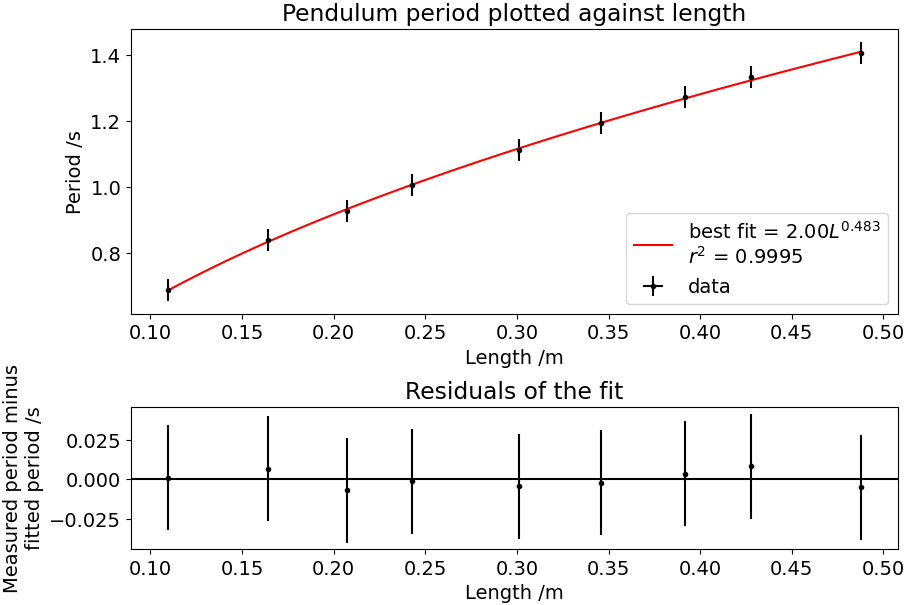
\includegraphics[width=\textwidth]{../figures/period_vs_length.png}
    \caption{\centering Graph of pendulum period plotted against pendulum length}
    \label{fig:figure 6}
\end{figure}

The uncertainty for length (0.1\,cm) was taken to be twice the smallest increment of a tape measure since a double-ended measurement was used to determine pendulum length. As in previous sections, the uncertainty for a period was taken to be 1/30\,s.

\newpage

\subsection{Analysis}
Equation \ref{eq:l-over-g} can also be represented in the form of $T = AL^n$ where $A = 2\pi/\sqrt{g} \approx 2$ and $n = 0.5$. This equation is displayed as the line of best fit in Figure \ref{fig:figure 6}, which also determines the uncertainty of $A = 0.01$ and $n = 0.004$.

The $r^2$ value for this fit, combined with consistent and low residuals implies that for small angles, the relationship between period and length is governed by Equation \ref{eq:l-over-g}.

To further prove that the line of best fit represents a square root function, Figure \ref{fig:figure 6} may be replotted with a log-log graph, shown below:

\begin{figure}[!hptb]
    \centering
    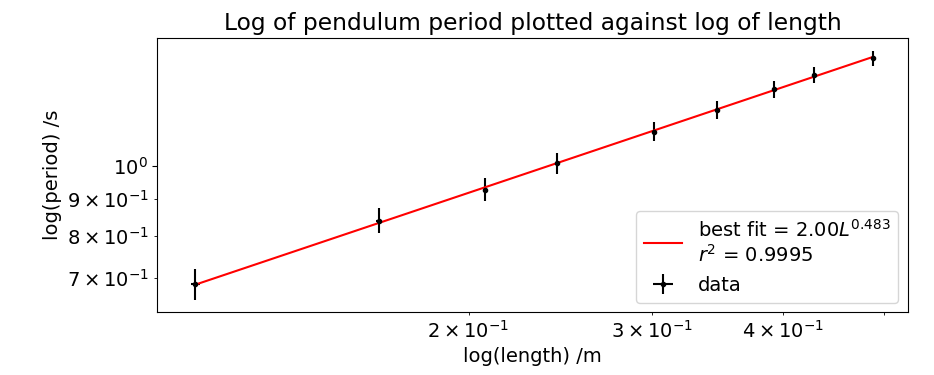
\includegraphics[width=\textwidth]{../figures/period_vs_length_log.png}
    \caption[]{Figure \ref{fig:figure 6} plotted with a log-log graph}
    \label{fig:figure 7}
\end{figure}

Given Equation \ref{eq:l-over-g}, taking log on both sides results in an equation in the form of $y = mx + b$ where the slope of the line $m$ equals to the power $n$. Plotting on a logarithmic axis provides a useful way to analyze functions that obey a power law, where the adjusted line of best fit should look linear, as expected in Figure \ref{fig:figure 7} reinforcing the idea that Equation \ref{eq:l-over-g} is an accurate way of representing the relationship between pendulum period and length.

\section{Q Factor and Length}

\subsection{Experimental Setup}
The same setup from Section \ref{Finding the Q Factor} was used to calculate the Q factors. Videos of the pendulum were not just recorded to include a few swings for Section \ref{Period and Length}, but rather up to hundreds of swings to capture the complete dampening effect of the pendulum.

\newpage

\subsection{Data}
The Q factor for every length was calculated by using Equation \ref{eq:q-factor-formula} with generated values of $\tau$ and $T$ as demonstrated in Section \ref{Finding the Q Factor} because the uncertainty is smaller in general. the Q factors for all 9 lengths is shown below with a line of best fit:

\begin{figure}[!hptb]
    \centering
    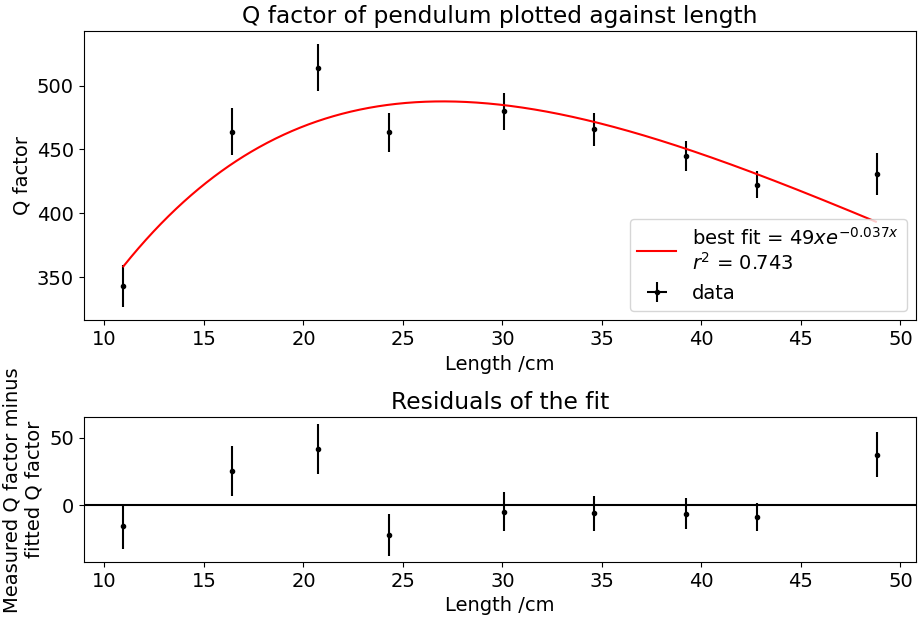
\includegraphics[width=\textwidth]{../figures/qfactor_vs_length.png}
    \caption{\centering Graph of Q factor plotted against pendulum length}
    \label{fig:figure 8}
\end{figure}

\subsection{Analysis}
The Q factor seems to peak at a certain point, which could be explained by the following. When the pendulum length is small, the force of air resistance plays less of a role than the force of friction at the end of the string and within the string fibers. When the pendulum length is long, the force of air resistance plays more of a role than all forces of friction within the string. This is because for a longer string released at the same angle as a smaller string, more gravitational potential energy gets converted to kinetic energy, implying a higher speed and even higher force of drag since its porportional to $v^2$ \cite{airdrag}. Additionally, the weight of the string starts to not be negligible when the pendulum length is long, as the pendulum stop behaving like a simple pendulum and the string also contributes to a surface area that experiences drag.

Modelling the Q factor graph in terms of a exponential, quadratic, sinusoidal, or power law function makes zero sense because intuitively, the Q factor should be 0 when the string length equals 0, and the Q factor should approach 0 when the string length is extremely long. A function that seems to satisfy these constraints is given by\footnote{a full derivation for this equation is found in the appendix}
\begin{equation} \label{eq:crit-damp}
    Axe^{-bx}
\end{equation}
which comes from the general shape of a critically damped oscillating system \cite{crit-damping}, modelling the Q factor graph somewhat nicely with a relatively low $r^2$ value of 0.750

Unfortunately, it cannot be concluded that \ref{eq:crit-damp} is the correct model to represented Q factor in terms of length due to the use of intuition, but it can be concluded that Q factor does depend on pendulum length.
}

\newpage

\printbibliography[heading=bibintoc]

\newpage

\appendix

\section{Q Factor Derivation}
Q factor is total oscillations until amplitude decays to $e^{-\pi}\theta_0$.

\begin{align*}
    \text{total oscillations} = Q \times \frac{\text{energy lost}}{\text{1 oscillation}} &= \text{total energy lost} \\
    \implies \quad Q &= \frac{E_T}{E_{osc}}
\end{align*}

Assuming that the energy lost per oscillation is constant \\

total energy loss to decay is equal to the difference in gravitational potential energy from $\theta_0$ to $e^{-\pi}\theta_0$ since from the following diagram:
<labelled pendulum diagram here or can just say determine geometrically> \\

also redefine $e^{-\pi}\theta_0 = \theta_f$

\begin{align*}
    E_T &= mgL(1-\cos\theta_0) - mgL(1-\cos\theta_f)\\
    &= mgL(\cos\theta_f-\cos\theta_0)
\end{align*}

previous equation implies that $E_T \propto L$

\begin{equation}
    E_T = c_1 L
\end{equation}

Now energy loss per oscillation - the forces that are doing the work are friction and air resistance

taking the pendulum diagram again, where $\theta_1$ = angle of pendulum after 1 oscillation

\begin{equation}
    mgL(1-cos\theta_0) = mgL(1-cos\theta_1) = W_{f} + W_{d}
\end{equation}

more assumptions -> from differential equation to solve for harmonic oscillator we know that $F_f \propto \frac{d\theta}{dt} = \omega$

since $\omega = \frac{2\pi}{T}$ and also Equation \ref{eq:l-over-g}, $\omega \propto \frac{1}{\sqrt{L}} \implies F_f \propto \frac{1}{\sqrt{L}}$

Work = $F\times d$ and $d = L(\theta_0 - \theta_1) = \text{arc length}$, therefore

\begin{align}
    W_f &= F_f L(\theta_0 - \theta_1) \\
    &\propto \frac{L}{\sqrt{L}} \\
    &= c_2\sqrt{L}
\end{align}

For the air resistance, we know that $F_d = \frac{1}{2}\rho C_d A v^2$. However $v^2$ is simply $(\omega L)^2 = \left(\frac{2\pi}{T(L)} L\right)^2 = k_1L$. $\rho$ and $C_d$ doesn't change for the pendulum. $A$ changes with length - this is because as the string gets longer, the total surface area increases. With the increase in length, the drag force on the string along is porportional to its length, but the surface area of the bob must also be taken into account, resulting in the area exposed to air for pendulum to be equal to $(Lw + A_{bob})$, where $w$ is the width of the string, which does not change. Thus,

\begin{equation}
    F_d = \frac{1}{2}\rho C_d (Lw + A_{bob}) k_1L
\end{equation}

Then the work done is represnted by
\begin{align*}
    W_d &= F_d L(\theta_0 - \theta_1) \\
    &= c_4L^2(L+c_3)
\end{align*}

Thus, the final equation for Q factor is represented by the equation
\begin{align}
    Q(L) &= \frac{c_1L}{c_2\sqrt{L} + c_4L^2(L+c_3)} \\
    &= \frac{d_1L}{d_2\sqrt{L} + L^2(L+d_3)}
\end{align}

where $d_1$, $d_2$, and $d_3$ are new constants after dividing the top and bottom by $c_4$.








\end{document}
